\setcounter{section}{3}
\setcounter{subsection}{6} % 3.7
\subsection{Analyse Ethernet-Rahmen}

Erzeugen Sie in einem geeignetem Netzwerkszenario Ethernet-Traffic und zeichnen
Sie diesen mit Wireshark auf
\begin{enumerate}[(a)]
    \item Finden Sie die Source und Destination MAC-Adresse im Ethernet-Header.
        Von welchem Hersteller stammen die Netzwerkkarten?

        Siehe Abbildungen~\ref{fig:3.7.a.destination} und \ref{fig:3.7.a.source}

        \verb|Destination, MAC-Adresse: b4:8c:9d::5d:14:01| \\
        \verb|Destination, Hersteller:  AzureWaveTec_5d| \\
        \verb|Source,      MAC-Adresse: 74:d4:35:af:19:77| \\
        \verb|Source,      Hersteller:  GigaByteTech_af|

    \item Erzeugen Sie Unicast und Broadcast-Traffic. Woran erkennen Sie den
        Unterschied im Ethernet-Header?

        Siehe Abbildungen~\ref{fig:3.7.b.destination} und \ref{fig:3.7.b.source}

        Der Unterschied zwischen einem Unicast- und einem
        Broadcast-Ethernet-Rahmen liegt in der Destination-Adresse: Bei einem
        Broadcast wird beispielsweise für IPv4 die Adresse
        \verb|255.255.255.255| und für Ethernet \verb|ff:ff:ff:ff:ff:ff|
        verwendet. Neben dem allgemeinen Broadcast (255.255.255.255) gibt es
        auch sogenannte gerichtete Broadcast-Adressen, die auf ein bestimmtes
        Subnetz abzielen (z.B., \verb|5.9.1.255|).

    \item Welches Vermittlungsschicht-Protokoll ist in den Ethernet-Rahmen
        enthalten? Wo finden Sie diese Information im Ethernet-Header?

        Siehe Abbildungen~\ref{fig:3.7.c.protocol-frame} und \ref{fig:3.7.c.protocol-in-header}

        In dem Beispiel auf den Abbildungen wird das Protokoll IPv4 verwendet.
        Diese Information ist im letzten Feld des Headers zu finden, wie in der
        Abbildung hervorgehoben.

    \item Finden Sie alle Rahmen, bei denen Padding verwendet wurde. Wie groß
        ist der Rahmen?

        Siehe Abbildung~\ref{fig:3.7.d.padding}

        Mit Padding beträgt die Länge des Rahmens 60 Bytes.
\end{enumerate}


        % \verb|Destination, MAC-Adresse: 74:d4:35:af:19:77| \\
        % \verb|Destination, Hersteller:  GigaByteTech_af| \\
        % \verb|Source,      MAC-Adresse: d8:3a:dd:e1:f5:2f| \\
        % \verb|Source,      Hersteller:  RaspberryPiT_e1|

\begin{figure}[p]
    \centering
    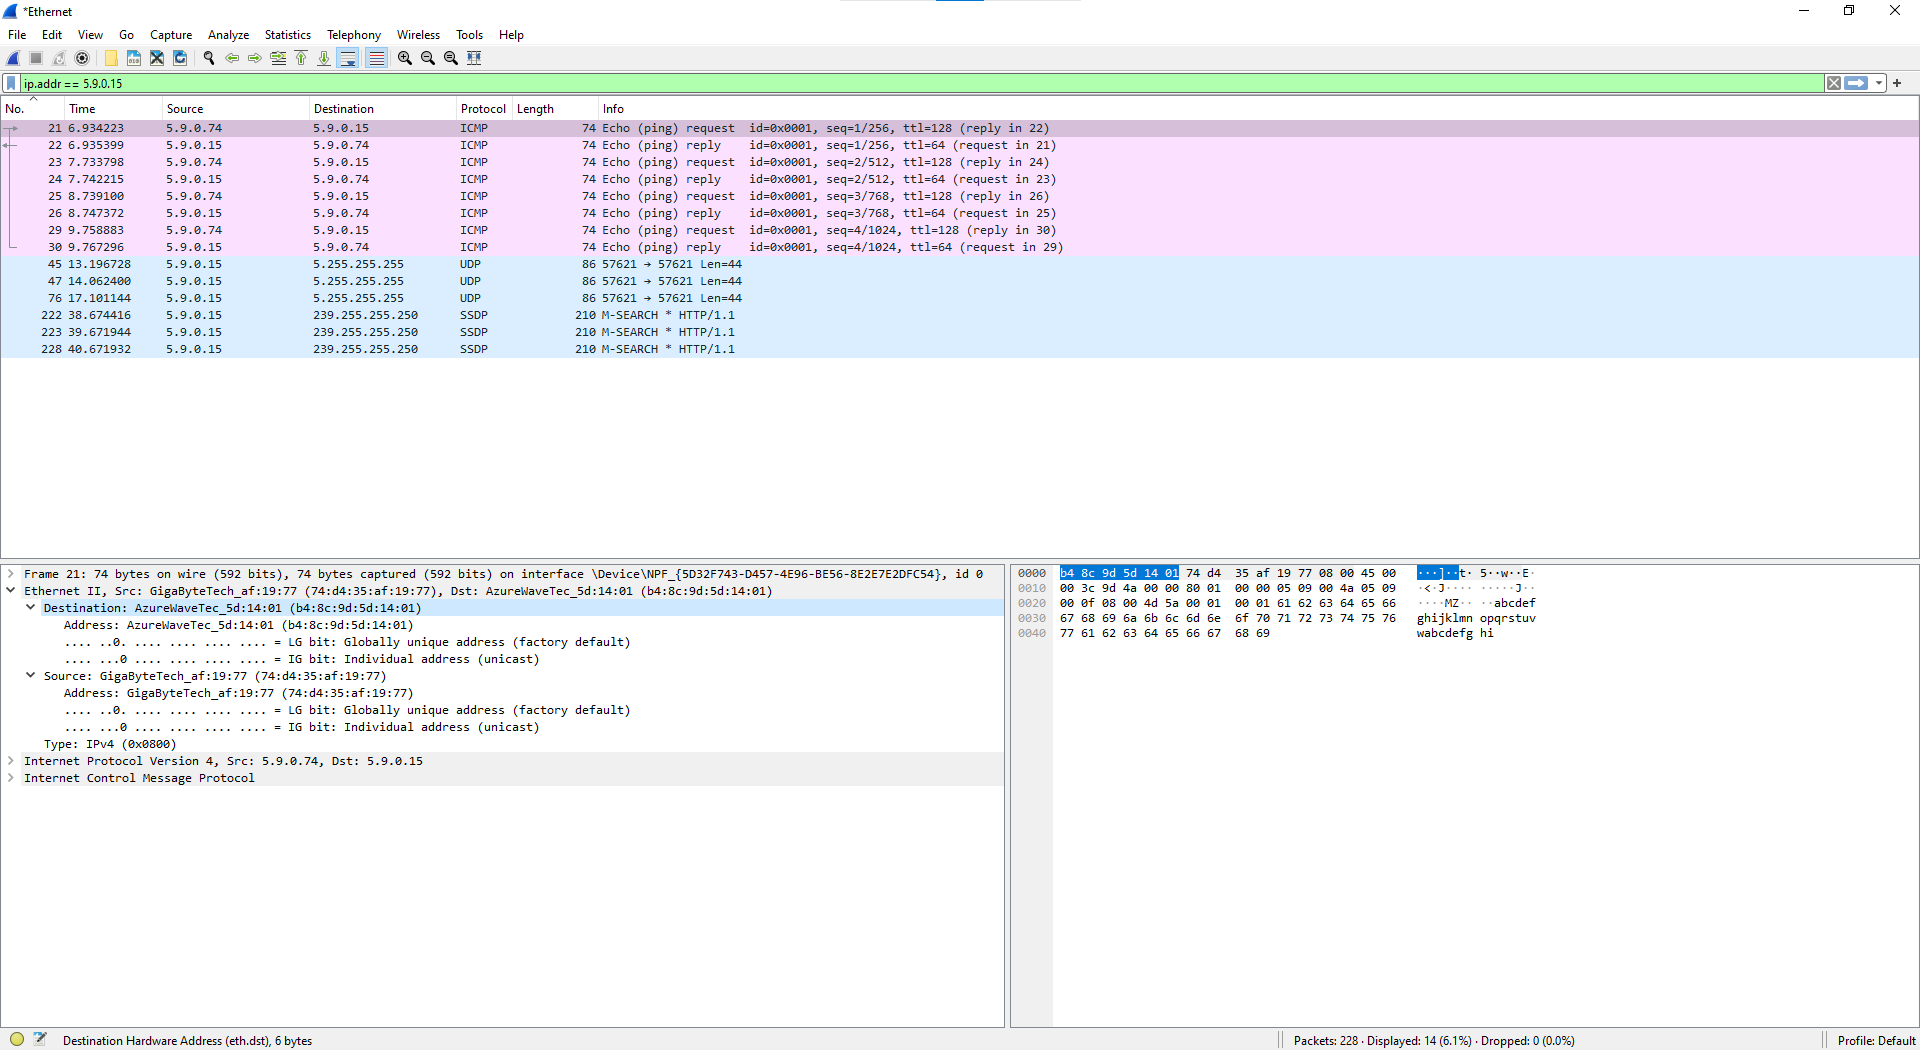
\includegraphics[width=1\textwidth]{./assets/3.7.a.destination.png}
    \caption{}
    \label{fig:3.7.a.destination}
\end{figure}

\begin{figure}[p]
    \centering
    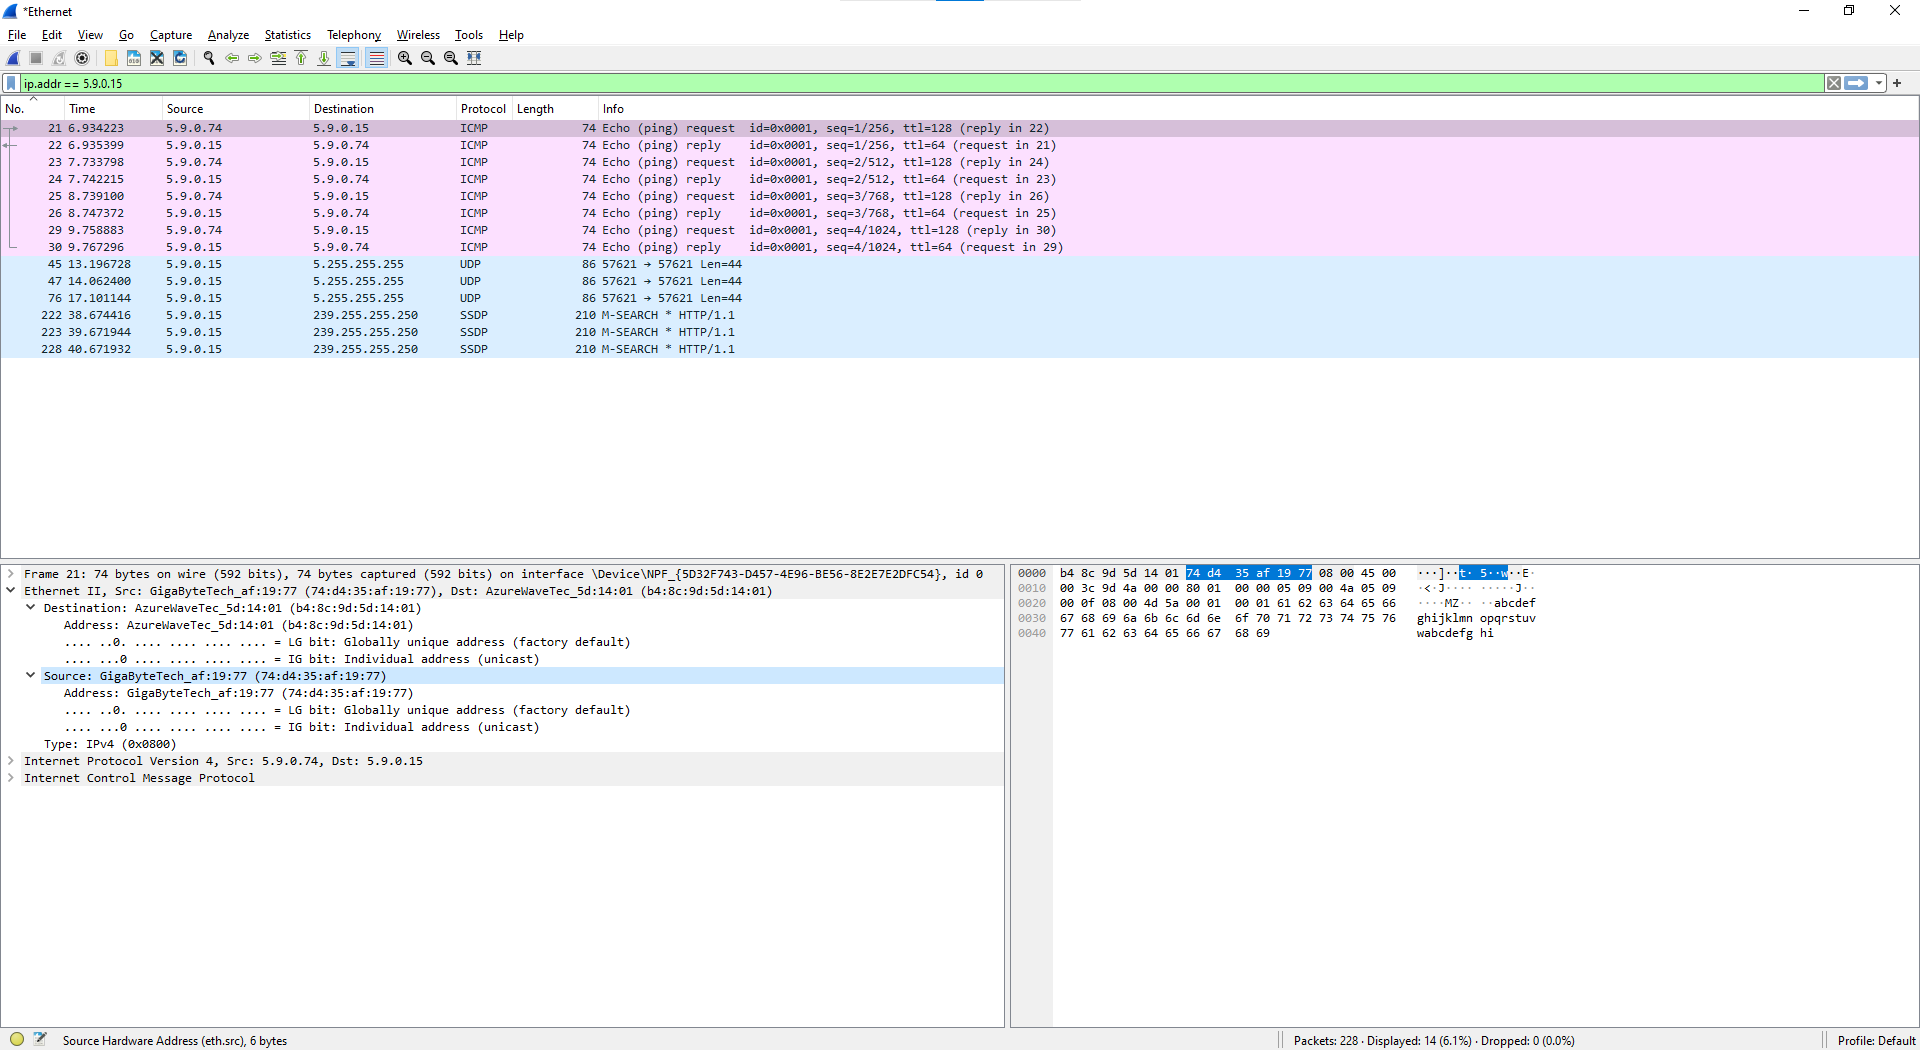
\includegraphics[width=1\textwidth]{./assets/3.7.a.source.png}
    \caption{}
    \label{fig:3.7.a.source}
\end{figure}

\begin{figure}[p]
    \centering
    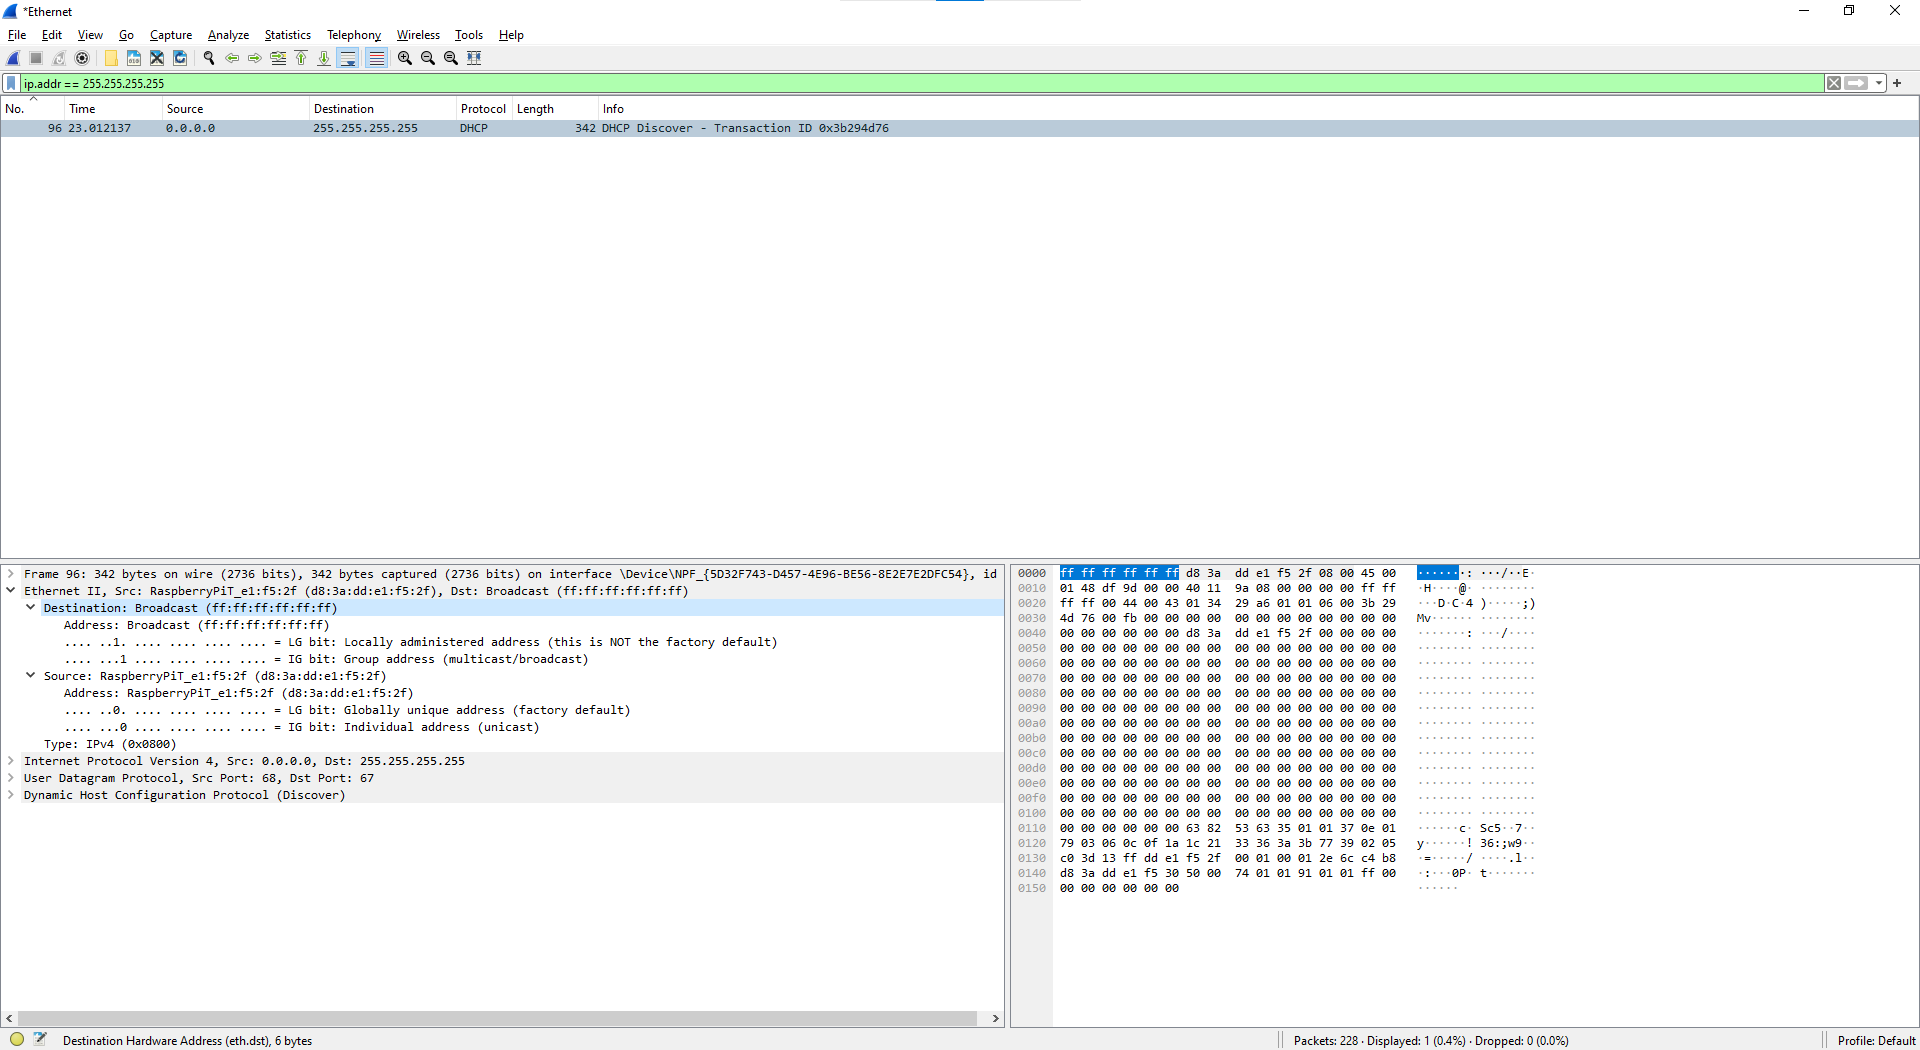
\includegraphics[width=1\textwidth]{./assets/3.7.b.destination.png}
    \caption{}
    \label{fig:3.7.b.destination}
\end{figure}

\begin{figure}[p]
    \centering
    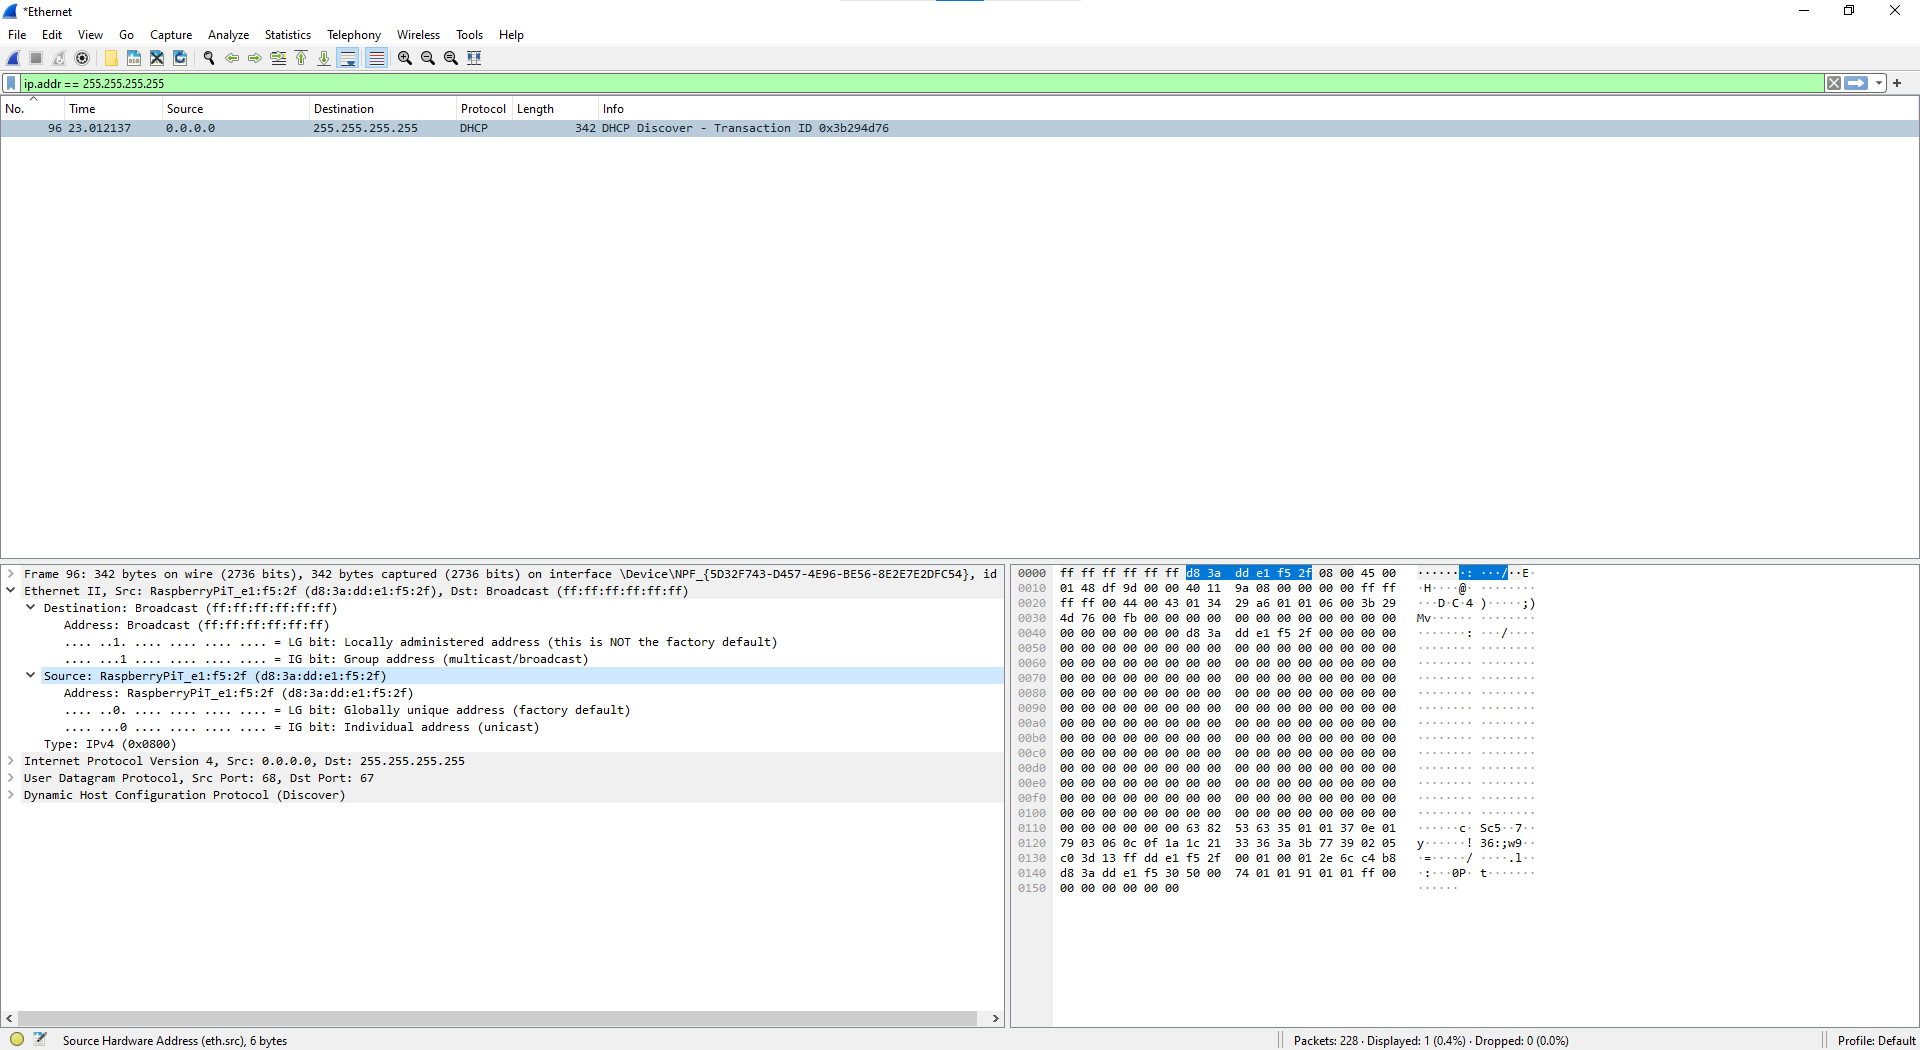
\includegraphics[width=1\textwidth]{./assets/3.7.b.source.png}
    \caption{}
    \label{fig:3.7.b.source}
\end{figure}

\begin{figure}[p]
    \centering
    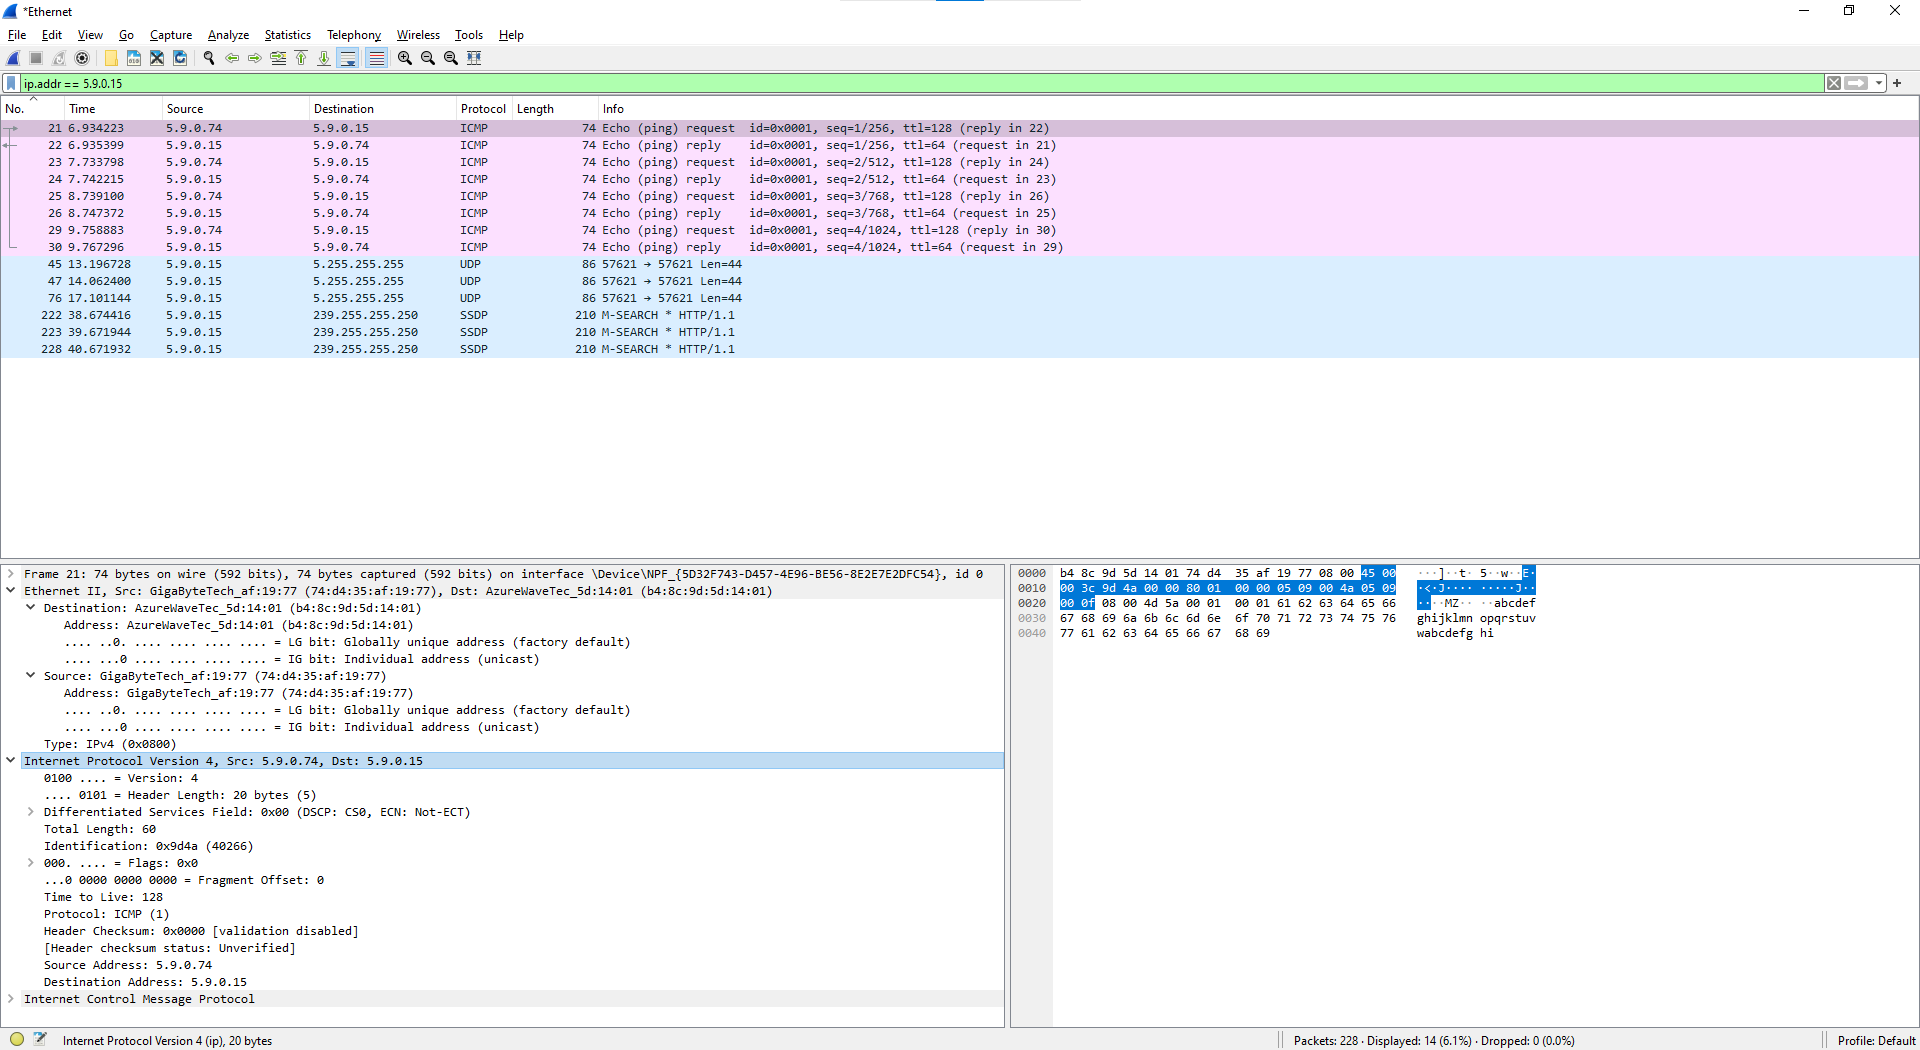
\includegraphics[width=1\textwidth]{./assets/3.7.c.protocol-frame.png}
    \caption{}
    \label{fig:3.7.c.protocol-frame}
\end{figure}

\begin{figure}[p]
    \centering
    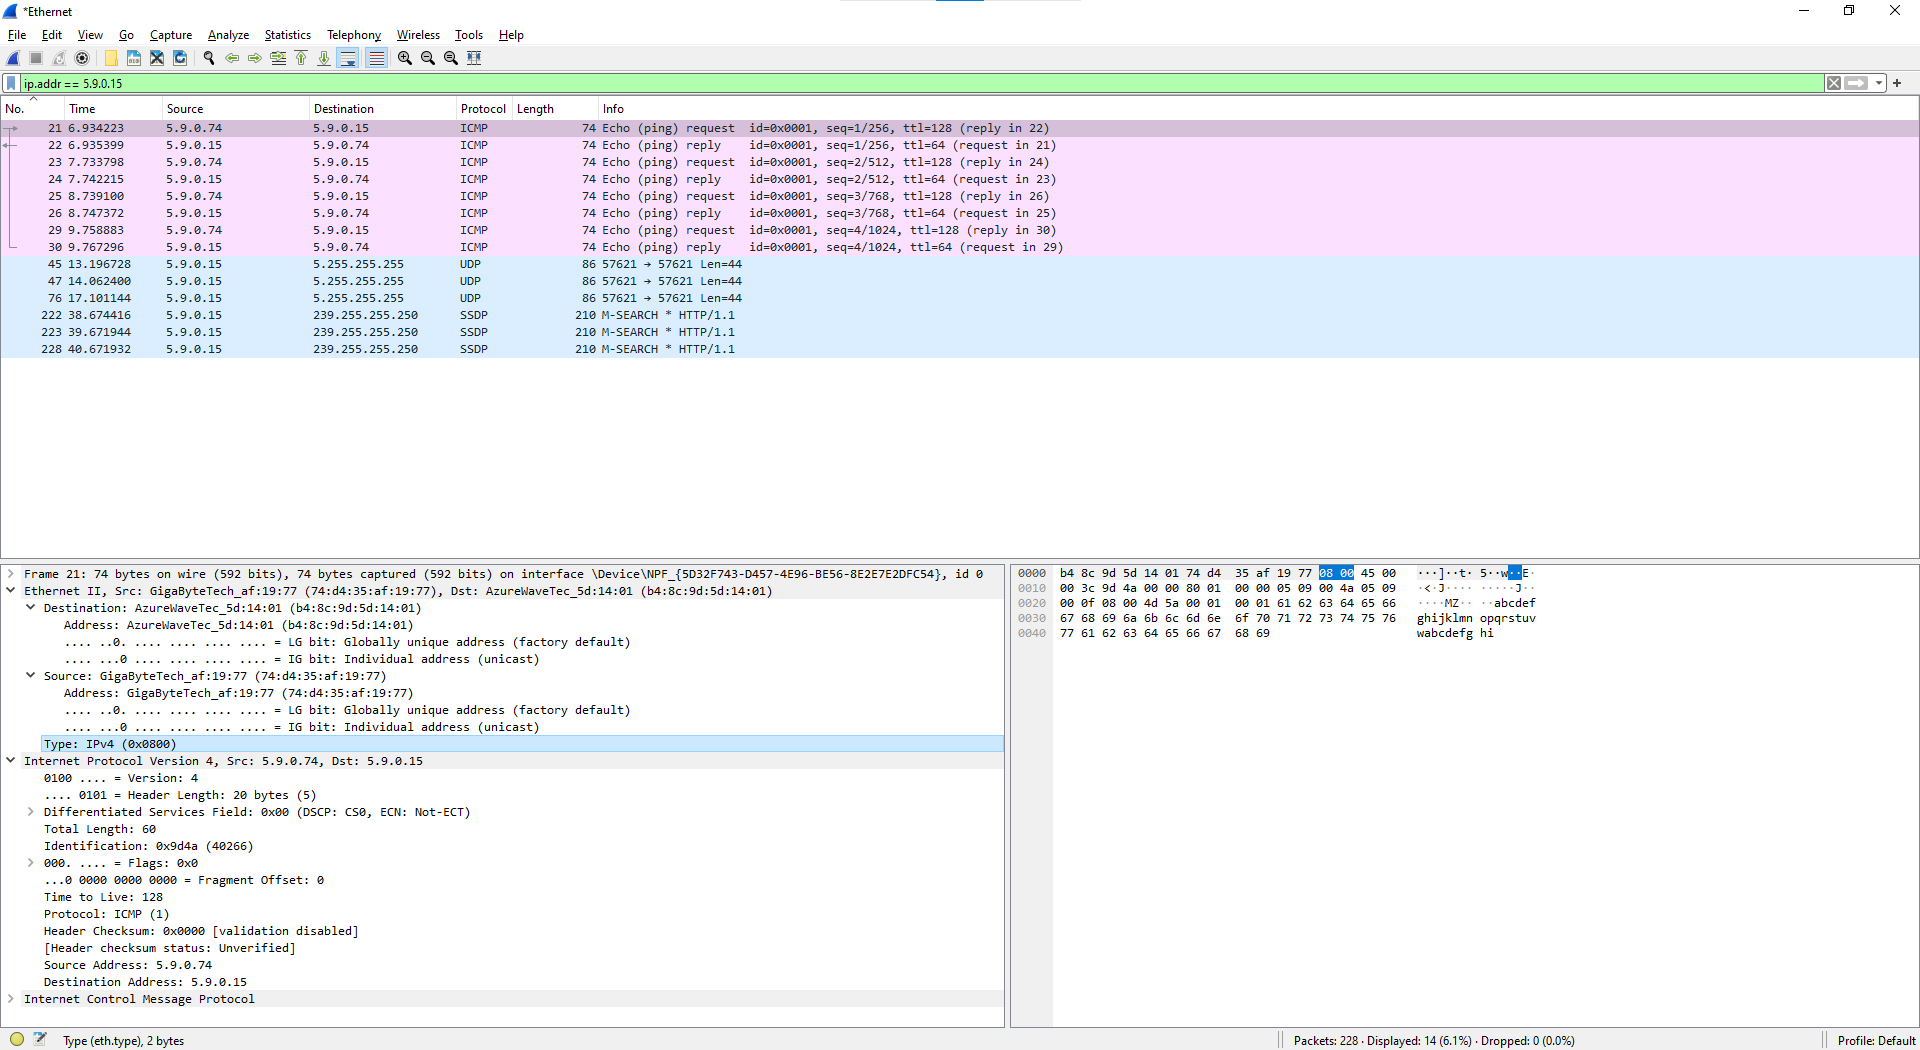
\includegraphics[width=1\textwidth]{./assets/3.7.c.protocol-in-header.png}
    \caption{}
    \label{fig:3.7.c.protocol-in-header}
\end{figure}

\begin{figure}[p]
    \centering
    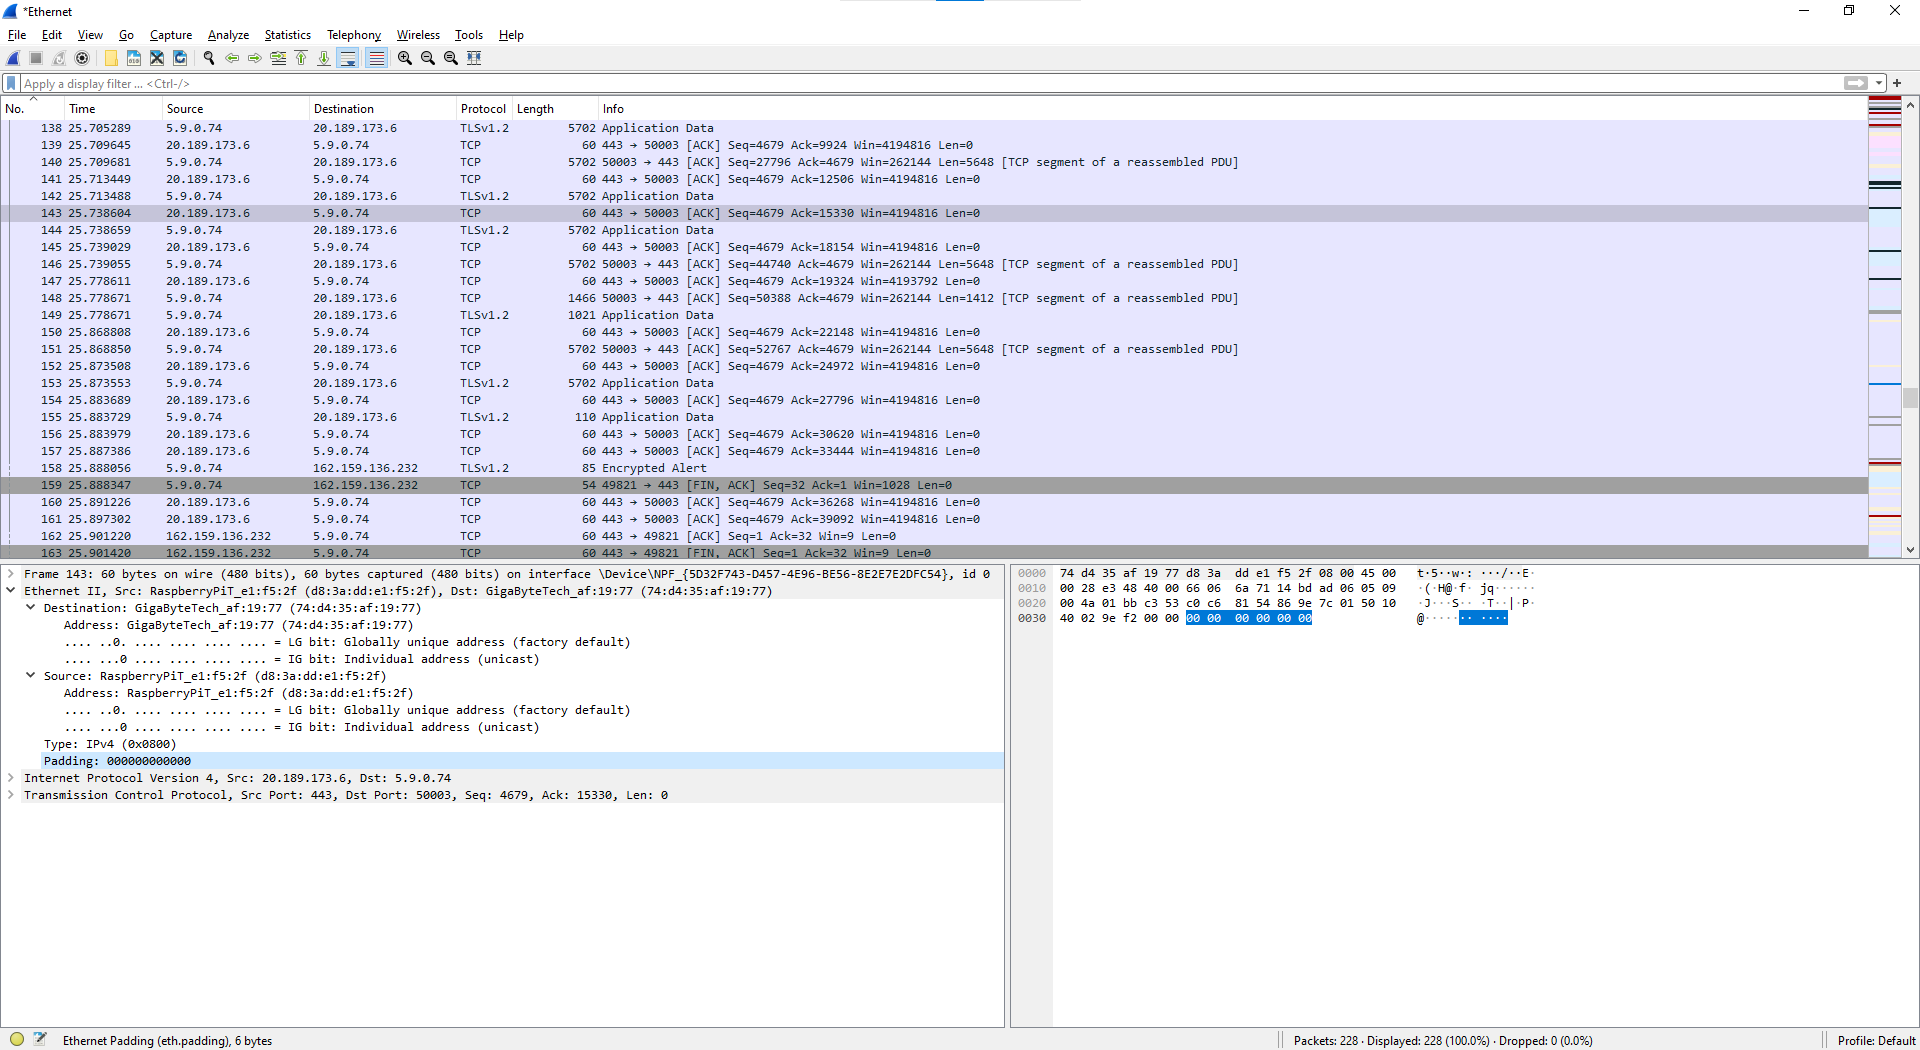
\includegraphics[width=1\textwidth]{./assets/3.7.d.padding.png}
    \caption{}
    \label{fig:3.7.d.padding}
\end{figure}

\FloatBarrier
